% CREATED BY DAVID FRISK, 2016
\chapter{Background}\label{chapter:background}
This chapter gives a short introduction to the technology used, as well as the different areas of knowledge needed to understand this thesis. For the technology, \textbf{Agda} and \textbf{Cubical Agda} are explained, as they provide the framework for the implementation. For the theory, a brief explanation of \textbf{Category Theory} is given, as well as some references to previous work on the main category of this thesis, \textbf{Poly}. Actually introducing the concepts of \textbf{Poly} is done in the theory section.

Some topics are not introduced in the background, but instead at the point where they are used. There is also a wealth of citations and references to deeper explorations of most concepts mentioned.

%and the different areas of knowledge used within the thesis. It explains \textbf{Agda} and \textbf{Cubical Agda} which provides the framework for the implementation. It also explains what \textbf{Category Theory} is, and finally giving some context of the main category of this thesis, \textbf{Poly}.


% This chapter gives a short introduction to the technology used and different areas of knowledge that is needed to understand this thesis. Starting with explaining \textbf{Agda}, which is the programming language used for the formalization. Going on to \textbf{Cubical Agda} which is an extension to \textbf{Agda} providing useful constructs aiding in writing proofs. Then to \textbf{Category Theory}


% This chapter explains any background needed to understand this thesis. 

% the decisions made prior to starting the work - namely what technology to use, why, and what to use it for. We will also dedicate a brief effort to explaining the basics of category theory and its mechanisms for generalizing and illuminating the subjects it's applied to. Finally, we'll briefly explore the specific category of polynomial functors - \textbf{Poly}, its surprising amount of structure and numerous interpretations in many different contexts - in other words, we will explain why this work was done and why we believe \textbf{Poly}, and polynomial functors in general, to be important.

\section{Agda}
Agda is a dependently typed programming language \cite{agdaWebsite} created at Chalmers. It is a functional language, with very similar syntax to Haskell, but with a more powerful type system which allows it to be used as a proof assistant. Dependent types means that types can depend on values. For example, it is possible for a function to have the type signature \mintinline{agda}{natOrBool : (b : Bool) → if b then ℕ else Bool}, which means it returns a natural number if the value of the argument is true, and a boolean if the value of the argument is false. In a non-dependent language, this would need to be expressed at the value level, so the function would have to return a value of type \mintinline{haskell}{Either ℕ Bool}.

\subsection{Unicode characters}
Agda, compared to most other languages, allows, and makes heavy use of unicode characters in symbol names. This can look daunting, but allows for a concise syntax more akin to mathematical notation. 

\subsection{Propositions as Types}
The Curry-Howard isomorphism \cite{propositionastypes} is the idea that there is a one-to-one correspondence between types in programming languages, propositions in logic, and expressions in algebra. Under this correspondence (isomorphism), a value of a type can be seen as a proof of the proposition the type corresponds to \cite{DependentTypesAtWork}. For example, the following data type in Agda corresponds to the logical operator \texttt{or} (written $A \vee B$):

\begin{minted}{agda}
data Either (A B : Type) : Set where
    inj₁ : A → Either A B
    inj₂ : B → Either A B
\end{minted}

It takes two types as arguments, and produces another type as an argument - much like the proposition $A \vee B$ is constructed out of the two propositions $A$ and $B$. This in turn also corresponds to summing in algebra - $A + B$. A summary of the isomorphism is given below:

\begin{table}[]
\begin{tabular}{lll}
Algebra      & Logic                   & Types \\
$A + B$      & $A \vee B$              & \texttt{Either A B} \\
$A \times B$ & $A \wedge B$            & \texttt{Pair A B}\\
$B^A$        & $ A \implies B$         & \texttt{A -> B} \\
$A = B$      & $ A \iff B$             & \texttt{Iso A B}
\end{tabular}
\end{table}

Concretely, an element of type \texttt{Either A B} is either an element of \texttt{A}, contained in the first value constructor \texttt{inj₁}, or of the type \texttt{B}, contained in the second value constructor \texttt{inj₂}. This corresponds to the fact that that a proof of the logical proposition $A \vee B$ is either a proof of the proposition \texttt{A} or a proof of \texttt{B}.

The Curry-Howard isomorphism together with its powerful type system makes Agda a powerful proof checker.


\subsection{Agda examples}
The \mintinline{agda}{Either} example above shows how (polymorphic) datatypes are defined, which should be similar to the GADTs \cite{haskellGADT} extension of Haskell.

It is also possible to create record types, for data types with only one constructor.

\begin{minted}{agda}
record Action : Type where
  constructor mkAction
  field
    write : Alphabet
    move : Movement
\end{minted}

The unit type and unit function is defined as:
\begin{minted}{agda}
data ⊤ : Type where
    tt : ⊤

unit : {A : Type} → A → ⊤
unit _ = tt
\end{minted}

The bottom (or False) type, and the absurd function from bottom:
\begin{minted}{agda}
data ⊥ : Type where

absurd : {A : Type} → ⊥ → A
absurd ()
\end{minted}

The natOrBool function can be implemented as:
\begin{minted}{agda}
natOrBool : (b : Bool) → if b then ℕ else Bool
natOrBool true = 0
natOrBool false = true
\end{minted}

More explanations and examples of Agda can be found in \cite{agdaWebsite} and \cite{DependentTypesAtWork}. Otherwise, it should be possible to understand the more advanced concepts of Agda along the thesis.

\subsection{Foreign function interface - Haskell}
Agda has a fully-featured foreign function interface (FFI) with Haskell, providing access to the vast Haskell ecosystem. This is important to our application section, as it allows us to use well-established libraries for plotting graphs, writing versatile command-line interfaces, and fast matrix inversion. For a more detailed description of the supporting Haskell code and what it's used for, see \ref{app:haskell}.


%The programming language Agda is a natural choice for this project. Dependently typed programming languages allow for the expression of an incredibly vast array of mathematical concepts with the appropriate rigor, and Agda is a mature and robust language in this space. 

%It also has a fully-featured FFI to work with its compilation target, Haskell. This is important to our application work, where we sometimes need to use the Haskell ecosystem to produce things like plots and graphs and use BLAS-based matrix multiplication algorithms. 

% Further, Agda is developed within Chalmers, which allows us access to a great deal of expertise in the details of the language within the University.

\section{Cubical Agda}
Cubical \cite{cubicalAgdaDocs} is an extension to Agda bringing ideas from Homotopy Type Theory (HoTT) \cite{hottBook}. The main contribution of Cubical Agda is how to deal with equality.

Equality in normal Agda is defined as a datatype. However, this (propositional) equality has certain problems. For example, it is not possible to prove function extensionality, that two functions are equal if they are equal for all arguments. Functional extensionality, which is very useful, is directly provable in Cubical.

Cubical discards this datatype and uses its own notion of equality, the path. An equality between two elements $a : A$ and $b : A$ is a path from $a$ to $b$. In Cubical, this is achieved by a function $p : I \rightarrow A$ satisfying some conditions. Firstly, $I$ is a special type representing an interval or a path, ranging from $0$ to $1$. Secondly, the beginning of the path must be $a$, that is $p(0)=a$. Finally, the end of the path must be $b$, $p(1)=b$. The important thing to note is that given \mintinline{agda}{a b : A} a type \mintinline{agda}{a ≡ b} is really a function \mintinline{agda}{I → A} behind the scenes, satisfying the above conditions. 

The equality \mintinline{agda}{a ≡ b} is actually known as homogeneous equality, because $a$ and $b$ are of the same type. It is also possible to have an equality when $a$ and $b$ are of different types, named heterogeneous equality. In fact, homogeneous equality is a special case of heterogeneous equality, where $a$ and $b$ happen to be the same type. For this thesis, mostly equality between same types is used, so no further explanation of heterogeneous equality is needed.

It is also possible to combine Cubical Agda with propositional equality. Using the functions \mintinline{agda}{pathToEq} and \mintinline{agda}{eqToPath} it is possible to go back and forth between the two different notions of equality. Something that can be useful in some cases.

There exists a standard cubical library \cite{cubicalLibrary} which has plenty of constructs and proofs from HoTT. The Cubical library is extensively used in this project.

A useful property of Cubical Agda is that isomorphisms are the same as equalities. It is possible to go back and forth using \mintinline{agda}{isoToPath} and \mintinline{agda}{pathToIso}, from the standard Cubical library. This means that one way to prove an equality is to prove an isomorphism.

A final property, which is used heftily in this thesis is substition. Substitution makes it possible to transfer a property over an equality. The declaration of substitution, somewhat simplified, is 

\begin{minted}{agda}
subst : {A : Type} {x y : A} {B : A → Type} → (x ≡ y) → B x → B y
\end{minted}

The next subsection gives some more examples of Cubical Agda. Further information about Cubical Agda and HoTT can be found in  \cite{cubicalPaper} and \cite{hottBook}.

\subsection{Cubical examples}
The first example is to show that the absurd function, define before, is actually unique. Given any other function from the empty type, it is the same function as absurd. To show equality between functions, function extensionality is used. Finally, the lemma is easily proved by pattern matching on the empty type.

\begin{minted}{agda}
absurdUnique : {A : Type} → (f : ⊥ → A) → f ≡ absurd
absurdUnique f = funExt lemma
    where
        lemma : (x : ⊥) → f x ≡ absurd x
        lemma ()
\end{minted}

In propositional equality, \mintinline{agda}{refl} is the way to prove that any element $a$, is equal to itself. The function \mintinline{agda}{refl} can be recovered in Cubical as follows. Remember that this equality is a function from $I$ which must be $a$ at both endpoints, which it is, since it is constantly $a$ along the whole interval.

\begin{minted}{agda}
refl : {A : Type} → {a : A} → a ≡ a
refl {a = a} i = a
\end{minted}


% Cubical Type Theory \cite{cubical} is a setting in which the Univalence Axiom from Homotopy Type Theory is computable. In Agda, this allows certain constructs to be defined more directly and for the expression of their properties to be much simplified. An example of this is set quotients - Dependent Martin-Löf Type Theory tends to avoid set quotients to instead rely on setoids. However, to express notions like set coequalizers cleanly, one needs quotients, and Cubical Agda allows them to be simply definable as Higher Inductive Types - HITs.

% Another major benefit to our work that Cubical Agda provides is that function extensionality is provable in HoTT. Since we are working on categorical formalizations, we constantly want to prove equalities of arrows in \textbf{Poly}, a problem that will turn out to be proving equalities of dependent and non-dependent functions.

% Yet another benefit is that doing Category Theory in a HoTT setting is just \textit{nice}. In Category Theory, mathematicians are often careful to distinguish strict equality from isomorphism, but in HoTT this distinction conveniently vanishes. We make extensive use of this fact via the function \textit{isoToPath} from the Cubical library. The HoTT book goes in more detail on how to do a constructive category theory in the context of HoTT, and this talk https://www.youtube.com/watch?v=nalC40POVLU by David Jaz Myers, author of one of the main references of this thesis \cite{css}, explains in a more relaxed fashion as well. 

% There's also no loss of expressivity, since the Cubical library allows to convert back and forth between cubical and propositional equality via the functions \textit{pathToEq} and \textit{eqToPath}; another tool we use frequently.

% Finally, our supervisor Felix Cherubini is an experienced homotopy type theorist, on whose expertise we're happy to have been able to rely.

\section{Category Theory}

We make use of CT in this project in three different regards: we sometimes need to think about category theory in general and what is true in a pure context, sometimes how to apply categorical concepts to concrete scientific and engineering contexts, and sometimes on the syntactic issue of how to translate statements about CT to statements in Agda and its type theories. We will briefly expand on these three regards now.

\subsection{In general: pure and applied CT}

We think of Category Theory as the formal study of composition - meaning connecting two relationships to form a larger one. It has some axioms that always hold for its central object of study, which is categories themselves, and definitions that build on top of these axioms that allow a highly rigorous but simple form of abstract reasoning about either structures that exist within categories or between them. 

The definitions and associated axioms are extremely simple; a \textit{category} $\mathcal{C}$ consists of the following data:

\begin{enumerate}
  \item A collection of objects Ob($\mathcal{C}$) (we're careful to not say "\textit{set} of objects", to avoid size issues).
  \item For every two objects $A$ and $B$, a set of \textit{arrows} (also called \textit{morphisms} or simply \textit{maps}) between them denoted by $\mathcal{C}$(A , B). Individual arrows, when they need to be named, are represented like this: $f : A \rightarrow B $. This set is also called the \textit{hom-set}.
  \item For every object $A$, an identity arrow $id : A \rightarrow A$. Note that this means that the hom-set $\mathcal{C}$($A$ , $A$) is never empty, for any category: it must contain at least the identity arrow.
  \item A composition operator $ \circ $ , that gives rise to new arrows. For any three objects $A$, $B$ and $C$ and arrows $f : A \rightarrow B $ and $g : B \rightarrow C $, there exists an arrow $g \circ f : A \rightarrow C $. We read this as "g after f".
  
\end{enumerate}

And the following laws:

\begin{enumerate}
  \item $ \forall f. f \circ id = id \circ f = f $ (identity)
  \item $ \forall f\text{ }g\text{ }h. f \circ (g \circ h) = (f \circ g) \circ h $ (associativity of composition)
\end{enumerate}

The usual way of representing statements in category theory is through \textit{commuting diagrams}, like so:

% % https://q.uiver.app/?q=WzAsNCxbMCwxLCJBIl0sWzIsMSwiQyJdLFsxLDIsIkIiXSxbMSwwLCJEIl0sWzAsMiwiZiJdLFsyLDEsImciXSxbMCwzLCJoIl0sWzMsMSwiayJdXQ==
% \begin{tikzcd}
% 	& D \\
% 	A && C \\
% 	& B
% 	\arrow["f", from=2-1, to=3-2]
% 	\arrow["g", from=3-2, to=2-3]
% 	\arrow["h", from=2-1, to=1-2]
% 	\arrow["k", from=1-2, to=2-3]
% \end{tikzcd}

Here, the objects are $ A $, $ B $, $ C $ and $ D $, and the arrows are $ f : A \rightarrow B $, $ g : B \rightarrow C $, $ h : A \rightarrow D $ and $ k : D \rightarrow C $. Composite arrows and identity arrows are almost always omitted, but are always there implicitly. \textit{Commuting} means any path between two objects is the same, which in this case means  $ k \circ h = g \circ f $. In a sense, diagrams can be seen as category theory's analogue of abstract algebraic equations. Like equations handle symbols that can stand for anything, diagrams are a totally abstract representation of some structure in a category, containing objects and morphisms that are labeled and subject to constraints like being equal or unique, and should be interpreted as a statement.

In general settings of category theory, the meaning of the objects and arrows doesn't play any role - they are purposefully abstract. Concrete categories ought to have meaning to their arrows and what it means to compose them, like the category \textbf{Set}, where objects are sets and arrows are functions between them. They must also respect the laws to be categories of course. In our case, because the thesis has a large focus on applied category theory, we will also talk frequently about the meaning of the arrows and objects in \textbf{Poly} and some closely related categories; it's what makes them interesting after all.

Defining the main point of study of category theory is barely scratching the surface. There are many constructions and structures within the theory that we cannot explain in any detail that would do them justice here; instead we will introduce other concepts in CT as they become relevant.

We'll end this section by highlighting the fact that, although the definition of a category may not seem like much, it in a sense reveals \textit{the point} of category theory: it is a theory of \textit{compositionality}. What it means to compose relationships between objects, what facts are preserved under different compositions, how composing can generalize: this and other deep structural questions are at the core of this theory. 

It's in this spirit, of investigating compositionality, that \textit{applied} category theory is done. The main introductory textbook on the subject, \textit{Seven Sketches in Compositionality}, \cite{seven-sketches} does a good job of justifying this approach. The book usually starts with motivating examples in the real world, and what CT and its constructions and formalisms can bring to understanding them in better, or at least different ways. In our case this order is reversed; we present the theory first, but the goal of applying it is always present.


\subsection{In code: Agda's \texttt{agda-categories} library}

The poly-book demonstrates a large amount of category-theoretic constructs in the context of \textbf{Poly}, but we limit ourselves to the ones that are most essential. These tend to be quite ubiquitous, and as such, there are formulations of many of them in the Agda ecosystem: the three main ones we considered were the 1lab \cite{1lab}, the Cubical library's own \cite{cubical-cat}, and the \texttt{agda-categories} \cite{agda-cats} library. We choose the third one for a few reasons: firstly, it is very well documented, with a sensible user interface and active community. Secondly, it has more constructs: for example, it is the only one of the three in which exponential objects, a key feature of \textbf{Poly}, is present. Thirdly, it is interoperable with Cubical, since the definition of a category requires a user to provide an equivalence relation to express equality between arrows, where we can supply cubical equality.

The brunt of the work that \texttt{agda-categories} is doing for us is providing a general scaffolding for us to validate that our formalizations of the concepts in \textbf{Poly} are correct. Sometimes it also helps by providing pre-existing implementations of categories; for instance, polynomials are functors, and so we will often rely on the provided instance of the category of \textbf{Set} of sets and functions.

\section{Polynomial Functors}

The study of polynomial functors has an extensive literature in the pure category-theoretic setting, like the work of Joachim Kock \cite{kockpoly}\cite{kock2009polynomial}, but we follow the \textbf{poly-book} closely in this thesis. It is an applied category theory textbook, which means it consistently provides interpretations of abstract mathematical structures that correspond, mapping them to concrete concepts and applications. The most mature interpretations, as far as we can tell, are to database theory, decision systems, and dynamical systems. One of the authors of the book, David Spivak, has done work using \textbf{Poly} in the context of database theory \cite{spivak2023functorial}. The book spends some time developing intuitions on the decision-making perspective as well, but we could not find much work in this area. Finally, there's the interpretation of \textbf{Poly} in dynamical systems, which the book provides many examples of.

% \section{Figure}
% \begin{figure}[H]
% \centering
% 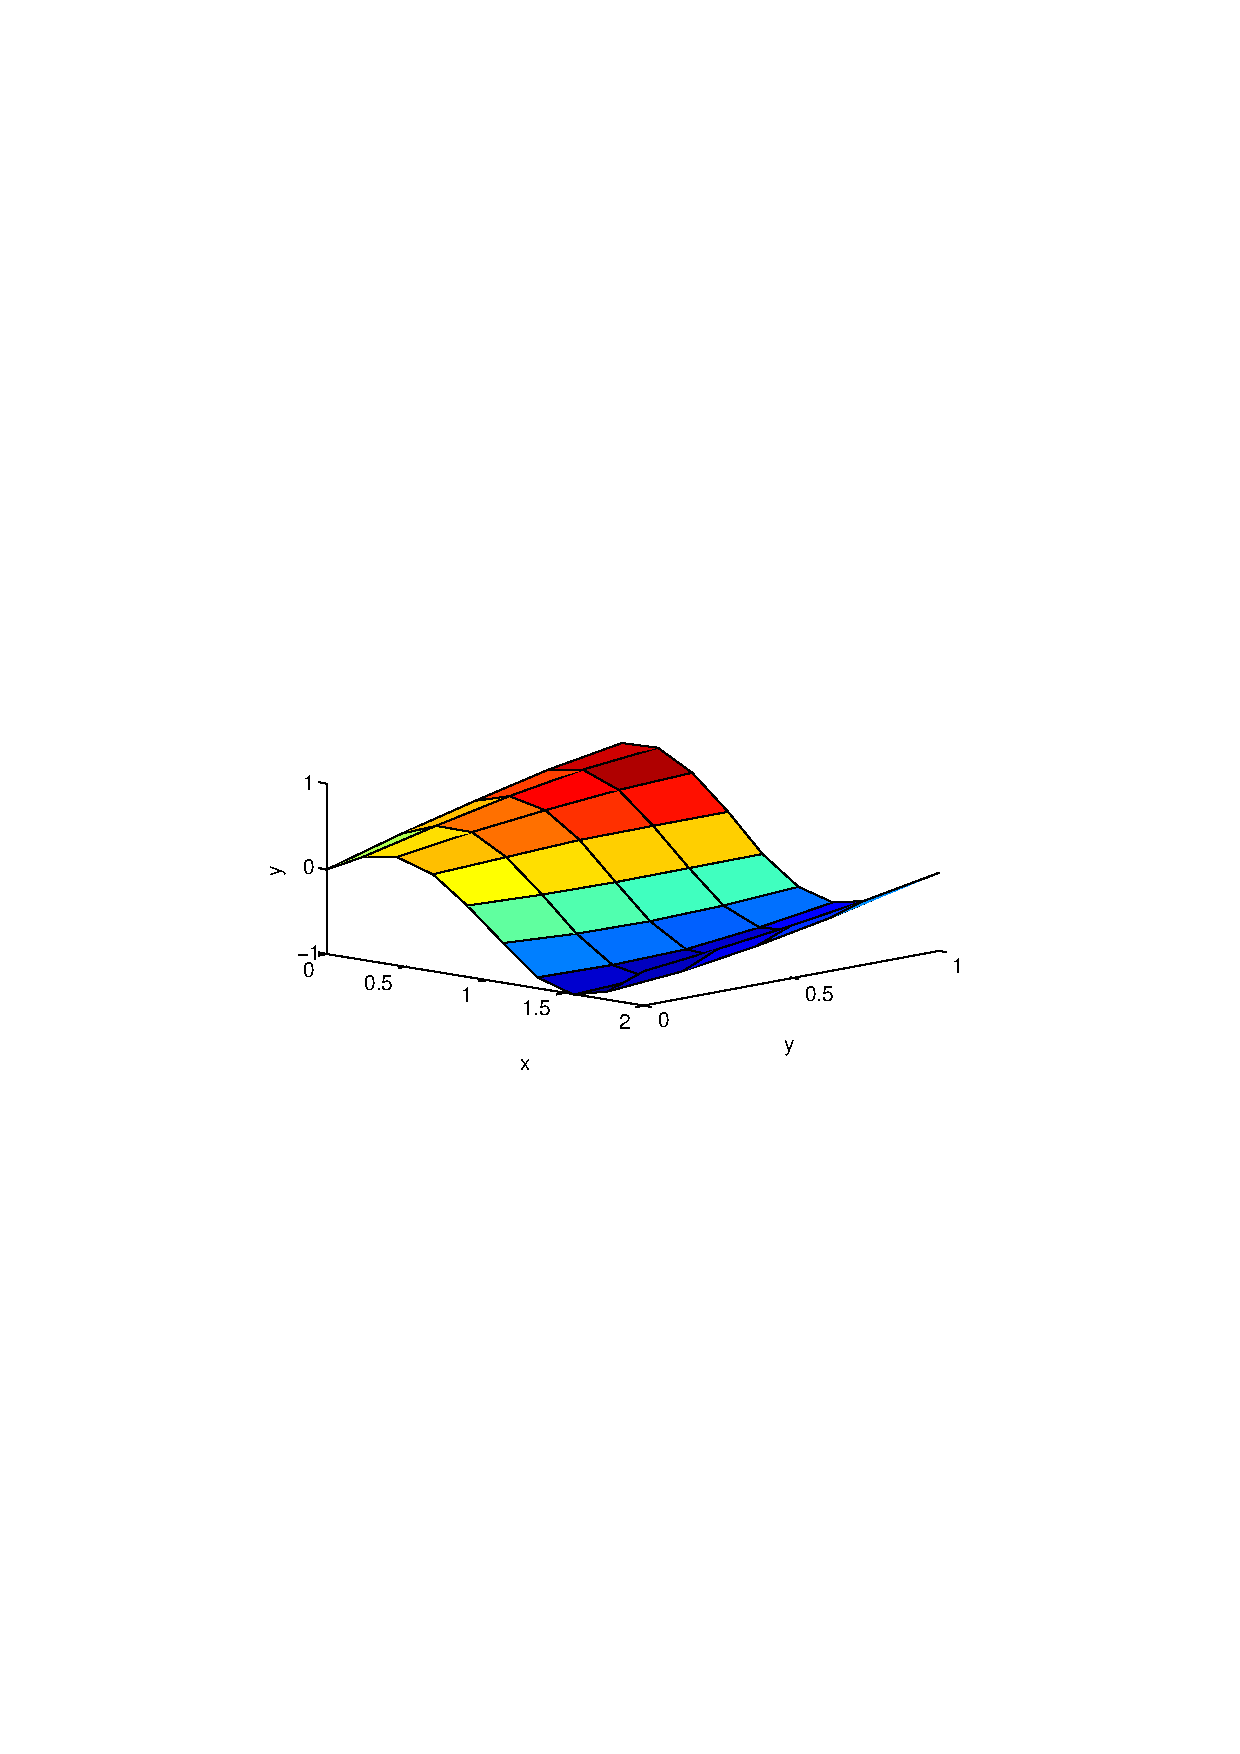
\includegraphics[width=0.45\linewidth, trim=3cm 11cm 3cm 11cm]{figure/X.pdf}
% 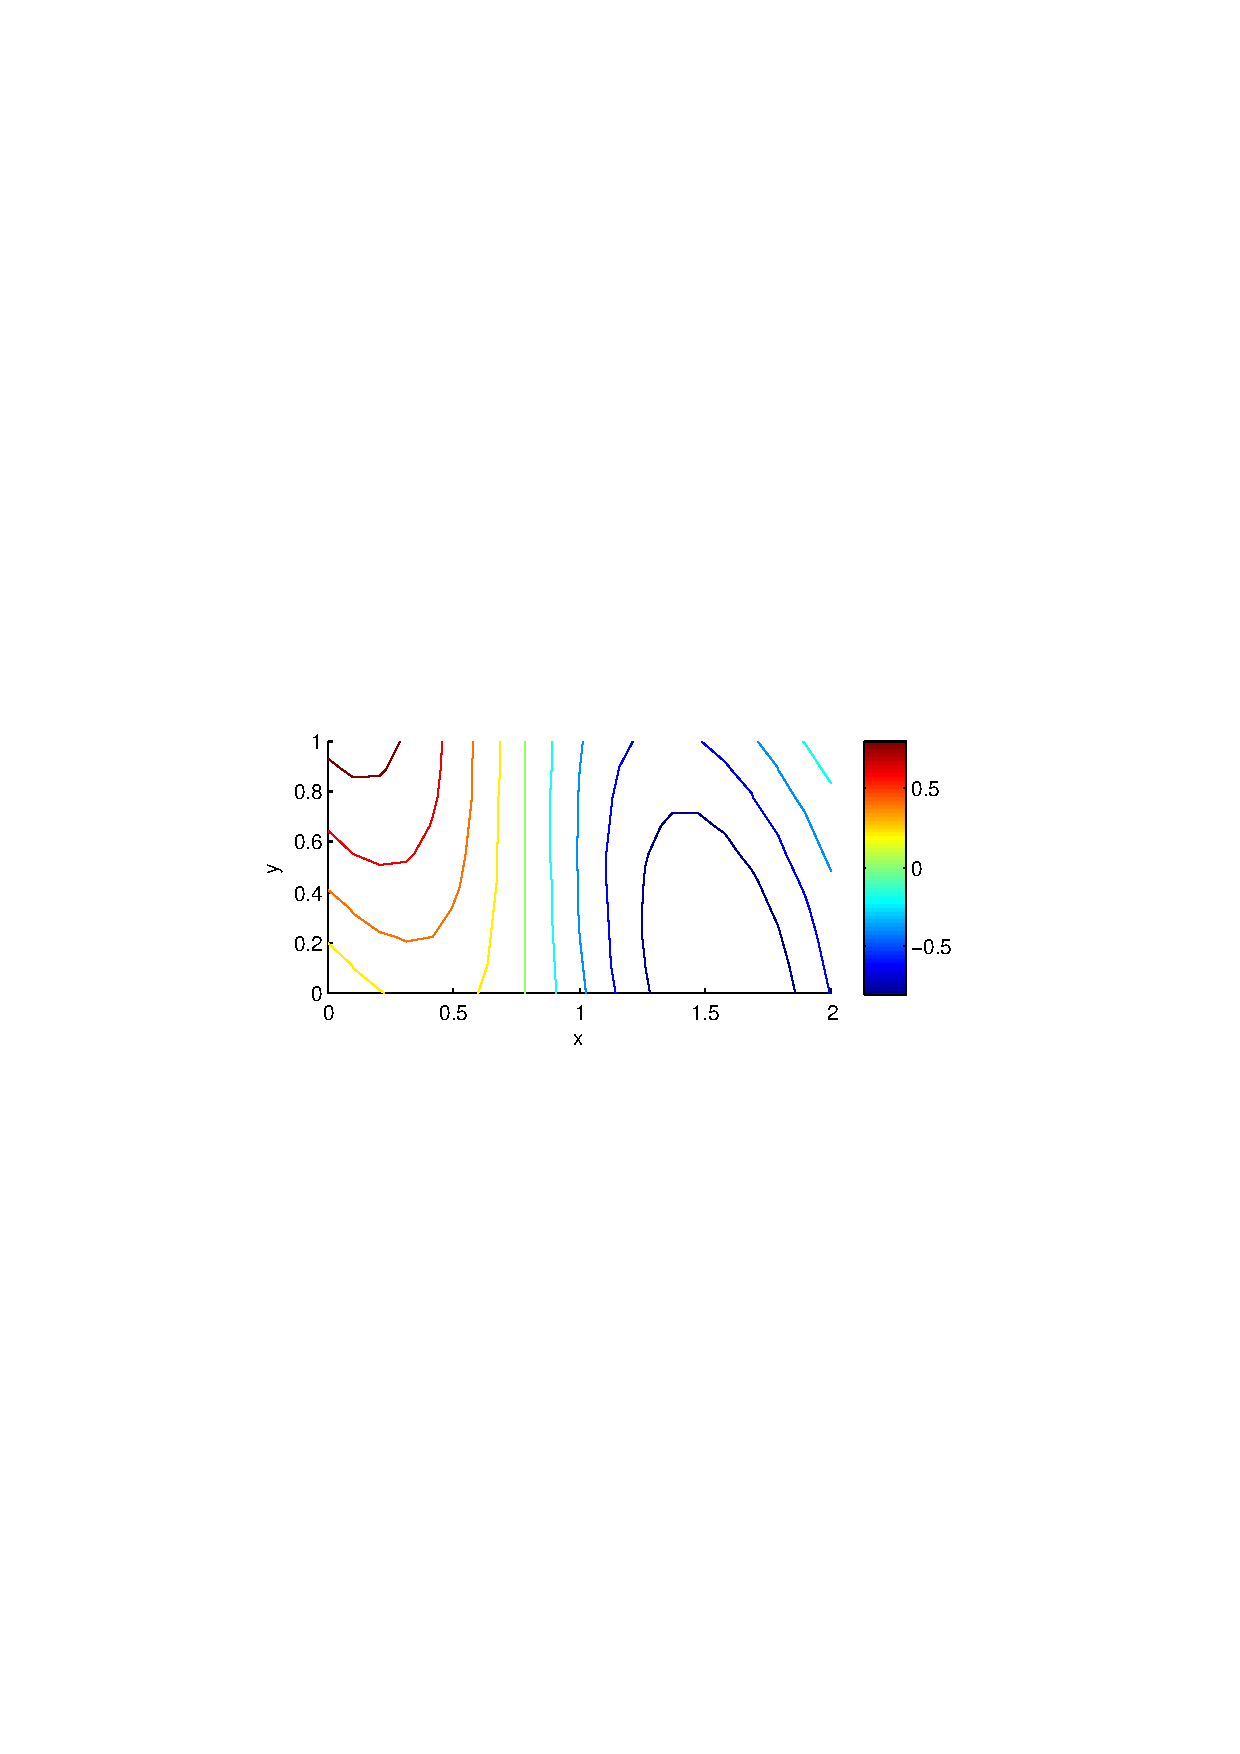
\includegraphics[width=0.45\linewidth, trim=3cm 11cm 3cm 11cm]{figure/Y.pdf}
% \caption{Surface and contour plots showing the two dimensional function $z(x,y)=\sin(x+y)\cos(2x)$.} % Figure text below figure
% \end{figure}
% 
% \section{Equation}
% \begin{equation}
% f(t)=\left\{ \begin{array}{ll}
% 1,~~~~ & t< 1 \\
% t^2 & t\geq 1
% \end{array}\right.
% \end{equation}
% 
% \section{Table}
% \begin{table}[H]
% \centering
% \caption{Values of $f(t)$ for $t=0,1,\dots 5$.}
% \begin{tabular}{l|llllll} \hline\hline
% $t$ & 0 & 1 & 2 & 3 & 4 & 5 \\ \hline
% $f(t)$ & 1 & 1 & 4 & 9 & 16 & 25 \\ \hline\hline
% \end{tabular}
% \end{table}
% 
% \section{Chemical structure}
% \begin{center}
% \chemfig{X*5(-E-T-A-L-)}
% \end{center}
% 
% 
% \section{Source code listing}
% \begin{minted}[frame=single]{matlab}
% % Generate x- and y-nodes
% x=linspace(0,1); y=linspace(0,1);
% 
% % Calculate z=f(x,y)
% for i=1:length(x)
%  for j=1:length(y)
%   z(i,j)=x(i)+2*y(j);
%  end
% end
% \end{minted}
% 
% \subsection{Other alternatives to the Theory chapter}
% Sometimes, it is more appropriate to name this chapter Background.
% 
% At CSE, there exists a large span of different types of thesis works. Sometimes it is more appropriate to join the Theory and Methods chapters, sometimes the Theory chapter would be so small that it should be a subsection. Talk to your supervisor to find the most appropriate structure for your thesis.